\documentclass{standalone}
\usepackage{tikz}
\usetikzlibrary{arrows.meta, bending}

\begin{document}

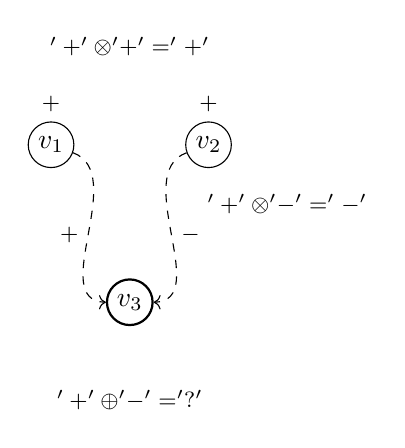
\begin{tikzpicture}
    % Nodes
    \node[circle, draw, inner sep=2] (v1) at (0, 2) {$v_1$};
    \node[circle, draw, inner sep=2] (v2) at (2, 2) {$v_2$};
    \node[circle, draw, thick, inner sep=2] (v3) at (1, 0) {$v_3$};
    
    % Edges and messages
    \draw[->, dashed] (v1) to [out=340, in=180] node[left, pos=0.5] {\footnotesize$+$} (v3);
    \draw[->, dashed] (v2) to [out=200, in=0] node[right, pos=0.5] {\footnotesize$-$} (v3);
    
    % Messages above
    \node[align=center, above] at (1, 3) {\footnotesize$'+' \otimes '+' = '+'$};
    \node[align=center, above] at (3, 1) {\footnotesize$'+' \otimes '-' = '-'$};
    
    % Messages below
    \node[align=center, below] at (1, -1) {\footnotesize$'+' \oplus '-' = '?'$};
    
    % Signs next to nodes
    \node[above] at (v1.north) {\footnotesize$+$};
    \node[above] at (v2.north) {\footnotesize$+$};
\end{tikzpicture}

\end{document}